\scanpage{44}
\mspage{\handwritten{12}}
\uline{Definition \handwritten{\makebox[0pt][l]{\raisebox{-2ex}{\unsure{\deleted{seen}|seen}}}}11.3.}- Given an $S$-group $G$ flat, quasi-compact and quasi-separated over $S$, such that $\handwritten{\unsure{\mathcal{A}|a}}(G)$ is flat over $\handwritten{\mathcal{O}}_S$, we shall denote by $G_{\mathrm{af}}$ , and shall call the \uline{affine envelope} of $G$ the $S$-group $G_{\mathrm{af}}=\operatorname{Spec}\handwritten{\mathcal{A}}(G)$.


\uline{\handwritten{\makebox[0pt][l]{\raisebox{-2ex}{\unsure{seen}}}}11.4.}- Given two quasi-coherent $\handwritten{\mathcal{O}}_S$-Modules $\handwritten{\mathcal{E}}$ and $\handwritten{\mathcal{F}}$, let us denote by $\handwritten{\mathcal{H}om}_S(\handwritten{\mathbb{V}}(\handwritten{\mathcal{F}}),\handwritten{\mathbb{V}}(\handwritten{\mathcal{E}}))$ the $S$-functor of morphisms of $S$-functors from $\handwritten{\mathbb{V}}(\handwritten{\mathcal{F}})$ to $\handwritten{\mathbb{V}}(\handwritten{\mathcal{E}})$, and by $\handwritten{\mathcal{H}om}_{\handwritten{\mathcal{O}}_S}(\handwritten{\mathbb{V}}(\handwritten{\mathcal{F}}),\handwritten{\mathbb{V}}(\handwritten{\mathcal{E}}))$ the sub-$S$-functor of $\handwritten{\mathcal{H}om}_S(\handwritten{\mathbb{V}}(\handwritten{\mathcal{F}}),\handwritten{\mathbb{V}}(\handwritten{\mathcal{E}}))$ formed by the $\handwritten{\mathcal{O}}_S$- homomorphisms of $\handwritten{\mathcal{O}}_S$-functors in modules (cf. \deleted{Lecture} I). Then $\handwritten{\mathcal{H}om}_{\handwritten{\mathcal{O}}_S}(\handwritten{\mathbb{V}}(\handwritten{\mathcal{F}}),\handwritten{\mathbb{V}}(\handwritten{\mathcal{E}}))(T)$ is in canonical bi\deleted{nu}\inserted{\handwritten{un}}ivocal correspondence with $\deleted{\unsure{\operatorname{Hom}}}\operatorname{Hom}_{\handwritten{\mathcal{O}}_{S\deleted{\unsure{T}}}\text{-}\mathrm{Mod.}}(\handwritten{\mathcal{E}\otimes}_{\handwritten{\mathcal{O}}_S}\handwritten{\mathcal{O}}_T,\deleted{\unsure{(}}\handwritten{\mathcal{F}\otimes}_{\handwritten{\mathcal{O}}_S}\handwritten{\mathcal{O}}_T\deleted{\unsure{)}}$,
\inserted{\handwritten{$\text{i.e.}\quad \mathcal{H}om_{\underline{O}_S}(\mathbb{V}(\mathcal{F}),\mathbb{V}(\mathcal{E}))\simeq\mathcal{H}om_{\underline{O}_S}(\mathbb{W}(\mathcal{E}),\mathbb{W}(\mathcal{F})).$}}


Let $X$ be an $S$-prescheme. Then the set of morphisms of $S$-functors from $X$ to $\handwritten{\mathcal{H}om}_S(\deleted{\handwritten{\unsure{\mathbb{V}|W}}}\handwritten{\mathbb{V}}(\handwritten{\mathcal{F}}),\handwritten{\mathbb{V}}(\handwritten{\mathcal{E}}))$ is in bi\inserted{\handwritten{un}}nnivocal correspondence with $\operatorname{Hom}_S(X\handwritten{\times}_S\handwritten{\mathbb{V}}(\handwritten{\mathcal{F}}),\handwritten{\mathbb{V}}(\handwritten{\mathcal{E}}))$, hence the set of morphisms of $S$-functors from $X$ to $\handwritten{\mathcal{H}om}_{\handwritten{\mathcal{O}}_S}(\handwritten{\mathbb{V}}(\handwritten{\mathcal{F}}),\handwritten{\mathbb{V}}(\handwritten{\mathcal{E}}))$ is in biunivocal correspondence with a subset of $\operatorname{Hom}_S(X\handwritten{\times}_S\handwritten{\mathbb{V}}(\handwritten{\mathcal{F}}),\handwritten{\mathbb{V}}(\handwritten{\mathcal{E}}))=\operatorname{Hom}_{\handwritten{\mathcal{O}}_S\text{-}\mathrm{Mod;}}(\handwritten{\mathcal{E}},\handwritten{\mathcal{A}}(X\handwritten{\times}_S\handwritten{\mathbb{V}}(\handwritten{\mathcal{F}})))$ (EGA II 1.7.13).

\uline{Proposition 11.5.- Let $X$ be an $S$-p\handwritten{\makebox[0pt][l]{\begin{tikzpicture}[x=.2cm,y=.2cm,baseline=-.3ex]\draw (0,-.2) .. controls (.35,0) and (.55,.4) .. (.8,.4);\end{tikzpicture}}}rescheme quasi-compact quasi-separated over $S$, $f:X\handwritten{\to}S$ the structure morphism, $\handwritten{\mathcal{E}}$ and $\handwritten{\mathcal{F}}$ two quasi-coherent $\handwritten{\mathcal{O}}_S$-Modules. We suppose that one of the following two conditions is satisfied\deleted{s} :}

\uline{a) $f$ is affine}

\uline{b) $\handwritten{\mathcal{F}}$ is flat over $\handwritten{\mathcal{O}}_S$.}

\uline{Then :}

\margin{\handwritten{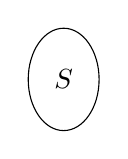
\begin{tikzpicture}\draw (0,0) ellipse (.45 and .65);\node at (0,0) {$S$};\end{tikzpicture}}}
\uline{i) the canonical homomorphism $\handwritten{\varphi:\mathcal{A}}(X)\handwritten{\otimes}_{\handwritten{\mathcal{O}}_S}\handwritten{\mathbb{S}}(\handwritten{\mathcal{F}})\handwritten{\longrightarrow\mathcal{A}}(X\handwritten{\times}_S\handwritten{\mathbb{V}}(\handwritten{\mathcal{F}}))$ is an isomorphism (where $\handwritten{\mathbb{S}}(\handwritten{\mathcal{F}})$ denotes the symmetric Algebra of $\handwritten{\mathcal{F}}$).}

\uline{ii) the set of morphisms of $S$-functors from $X$ to $\handwritten{\mathcal{H}om}_{\handwritten{\mathcal{O}}_S}(\handwritten{\mathbb{V}}(\handwritten{\mathcal{F}}),\handwritten{\mathbb{V}}(\handwritten{\mathcal{E}}))$ is in biunivocal correspondence with $\operatorname{Hom}_{\handwritten{\mathcal{O}}_S\text{-}\mathrm{Mod.}}(\handwritten{\mathcal{E}}\ ,\ \handwritten{\mathcal{A}}(X)\handwritten{\otimes\mathcal{F}})$.}

To show i), by (11.1, a) and b)), it suffices to show that if $\handwritten{\mathcal{F}}$ is flat over $\handwritten{\mathcal{O}}_{\unsure{\mathbb{S}|S}}$, \deleted{the same holds for $\handwritten{\mathbb{S}}(\handwritten{\mathcal{F}})$} then $\handwritten{\mathbb{V}}(\handwritten{\mathcal{F}})$ is flat over $S$. By (EGA III 1.4.15.5),
% archive sheet number: 43
